%Chapter 2
\chapter{Overview of simulation and compressed air applications}
\thispagestyle{empty}
\vspace{38em}
\hrulefill
\\
\enquote*{\textit{Quote.}} - Somebody\\
\clearpage
\section{Introduction}
\section{Review of compressed air energy interventions in industry}
	\subsection{Preamble}
		Compressed air improvement can be obtained through intervention in either the supply or demand of compressed air \cite{Kriel2014Masters}. Improvements in supply interventions are achieved by increasing the efficiency of compressed air supply. Examples of this type of intervention include \gls{dcs}, compressor maintenance, etc. 
		\par
		Due to the size of mining compressed air networks, there is often a larger scope for improvement in air demand. Improving the demand is achieved by optimising air flow consumers, reducing leaks, etc.
		\par
	 	 This section will review compressed air supply and demand interventions that have improved energy or operation efficiency the mining industry. From the, successes and shortcomings in studies will be discussed and analysed with regard to this study.
	 	
	\subsection{Strategies to improve compressed air supply}

		\subsubsection{Compressor efficiency improvements}
		\subsubsection{Optimising compressor control}
		Compressors types and numbers can differ widely from mining compressed air systems. Compressor selection is crucial in these systems to match the correct compressors with the requirements of the system \cite{marais2010expert}.
		\par 
		In a study by Booysen \textit{et al} \cite{Booysen2012Masters} on optimising compressor control, \cite{Booysen2012Masters} found that many mines control compressors using fixed target pressure points that are much higher that required. In one system, compressors were set to a target 650 \gls{kpa} to ensure pressure underground did not fall below 500 \gls{kpa}. Using high pressure set-points can lead to excessive wasteful blow-off flow when the pressure exceeds a maximum points.
		\par
		Booysen \cite{booysen2009optimising} showed that through dynamic pressure setpoint control, matching the supply pressure with the demand, and optimal compressor selection, energy savings can be achieved. In a case study, an average power reduction of 1.07 MW was achieved. The lead to an estimated energy cost saving of R3M.
		\par 
	 	Optimising control of compressors to match the demand of the system can be complicated. \glspl{vsd} and guide vain are used to control the capacity of the system. More effective power reductions can be achieved through the use of \gls{vsd} control. Running compressors at part load reduces efficiency. From literature it shown electric motors will typical use 60-80\% of there rated power when running at $<$50\% load \cite{Saidur2010}.
		
		%\subsubsection{Air storage}
		%- booysen 1.22
		%\subsubsection{Dynamic compressor selection}
		%- van Tonder PHD
		%- van heerden 
		
		\subsubsection{Reconfiguring compressed air networks}
			A number of old mining compressed air systems  have not been adequately maintained and improved. Often they cannot sufficiently supply air to meet the demand or air is provided from non optimal sources. In a study by Bredenkamp \cite{Bredenkamp2013Masters}, reconfiguring of the air network was investigated to improve these systems.
			\par  
			In the study, Bredenkamp investigated interconnecting the compressed air systems of two mining shafts and relocating of a compressor. This strategy lead to an average power reduction of 1.7 MW and an estimated annual energy cost saving of R8.9M at the time.
			\par 
			*** \textit{Discussion of Bredenkamp} shortcomings and successes ***
			
	\subsection{Strategies to reduce compressed air demand}
	As illustrated in \cref{fig: Mining schedule}
		- Reducing leaks\\
		- Marais PhD\\
		- Snyman - investigated various Compressed air demand reduction and efficiency
		 optimisations \cite{Snyman2011Masters}.
		 
		 \subsubsection{Leakage detection}
		 Air leaks are a major inefficiency in mining compressed air systems. Improving leaks is relatively easier method to  reduce air demand and improve the efficiency of the system  \cite{van2011sustaining}. Air leaks occur as a result of open pipes, fissure and breaks. Losses depend on the size of the leak. \cref{fig: Leak losses} shows the estimated power losses vs leakage area.
		 \par
		 ***Fix this  booysen 1.20 ***
		 \begin{figure}[h]
		 	\centering
		 	% GNUPLOT: LaTeX picture with Postscript
\begingroup
  \makeatletter
  \providecommand\color[2][]{%
    \GenericError{(gnuplot) \space\space\space\@spaces}{%
      Package color not loaded in conjunction with
      terminal option `colourtext'%
    }{See the gnuplot documentation for explanation.%
    }{Either use 'blacktext' in gnuplot or load the package
      color.sty in LaTeX.}%
    \renewcommand\color[2][]{}%
  }%
  \providecommand\includegraphics[2][]{%
    \GenericError{(gnuplot) \space\space\space\@spaces}{%
      Package graphicx or graphics not loaded%
    }{See the gnuplot documentation for explanation.%
    }{The gnuplot epslatex terminal needs graphicx.sty or graphics.sty.}%
    \renewcommand\includegraphics[2][]{}%
  }%
  \providecommand\rotatebox[2]{#2}%
  \@ifundefined{ifGPcolor}{%
    \newif\ifGPcolor
    \GPcolortrue
  }{}%
  \@ifundefined{ifGPblacktext}{%
    \newif\ifGPblacktext
    \GPblacktextfalse
  }{}%
  % define a \g@addto@macro without @ in the name:
  \let\gplgaddtomacro\g@addto@macro
  % define empty templates for all commands taking text:
  \gdef\gplbacktext{}%
  \gdef\gplfronttext{}%
  \makeatother
  \ifGPblacktext
    % no textcolor at all
    \def\colorrgb#1{}%
    \def\colorgray#1{}%
  \else
    % gray or color?
    \ifGPcolor
      \def\colorrgb#1{\color[rgb]{#1}}%
      \def\colorgray#1{\color[gray]{#1}}%
      \expandafter\def\csname LTw\endcsname{\color{white}}%
      \expandafter\def\csname LTb\endcsname{\color{black}}%
      \expandafter\def\csname LTa\endcsname{\color{black}}%
      \expandafter\def\csname LT0\endcsname{\color[rgb]{1,0,0}}%
      \expandafter\def\csname LT1\endcsname{\color[rgb]{0,1,0}}%
      \expandafter\def\csname LT2\endcsname{\color[rgb]{0,0,1}}%
      \expandafter\def\csname LT3\endcsname{\color[rgb]{1,0,1}}%
      \expandafter\def\csname LT4\endcsname{\color[rgb]{0,1,1}}%
      \expandafter\def\csname LT5\endcsname{\color[rgb]{1,1,0}}%
      \expandafter\def\csname LT6\endcsname{\color[rgb]{0,0,0}}%
      \expandafter\def\csname LT7\endcsname{\color[rgb]{1,0.3,0}}%
      \expandafter\def\csname LT8\endcsname{\color[rgb]{0.5,0.5,0.5}}%
    \else
      % gray
      \def\colorrgb#1{\color{black}}%
      \def\colorgray#1{\color[gray]{#1}}%
      \expandafter\def\csname LTw\endcsname{\color{white}}%
      \expandafter\def\csname LTb\endcsname{\color{black}}%
      \expandafter\def\csname LTa\endcsname{\color{black}}%
      \expandafter\def\csname LT0\endcsname{\color{black}}%
      \expandafter\def\csname LT1\endcsname{\color{black}}%
      \expandafter\def\csname LT2\endcsname{\color{black}}%
      \expandafter\def\csname LT3\endcsname{\color{black}}%
      \expandafter\def\csname LT4\endcsname{\color{black}}%
      \expandafter\def\csname LT5\endcsname{\color{black}}%
      \expandafter\def\csname LT6\endcsname{\color{black}}%
      \expandafter\def\csname LT7\endcsname{\color{black}}%
      \expandafter\def\csname LT8\endcsname{\color{black}}%
    \fi
  \fi
    \setlength{\unitlength}{0.0500bp}%
    \ifx\gptboxheight\undefined%
      \newlength{\gptboxheight}%
      \newlength{\gptboxwidth}%
      \newsavebox{\gptboxtext}%
    \fi%
    \setlength{\fboxrule}{0.5pt}%
    \setlength{\fboxsep}{1pt}%
\begin{picture}(9360.00,4032.00)%
    \gplgaddtomacro\gplbacktext{%
      \colorrgb{0.00,0.00,0.00}%
      \put(946,704){\makebox(0,0)[r]{\strut{}$0$}}%
      \colorrgb{0.00,0.00,0.00}%
      \put(946,1087){\makebox(0,0)[r]{\strut{}$1000$}}%
      \colorrgb{0.00,0.00,0.00}%
      \put(946,1470){\makebox(0,0)[r]{\strut{}$2000$}}%
      \colorrgb{0.00,0.00,0.00}%
      \put(946,1853){\makebox(0,0)[r]{\strut{}$3000$}}%
      \colorrgb{0.00,0.00,0.00}%
      \put(946,2236){\makebox(0,0)[r]{\strut{}$4000$}}%
      \colorrgb{0.00,0.00,0.00}%
      \put(946,2618){\makebox(0,0)[r]{\strut{}$5000$}}%
      \colorrgb{0.00,0.00,0.00}%
      \put(946,3001){\makebox(0,0)[r]{\strut{}$6000$}}%
      \colorrgb{0.00,0.00,0.00}%
      \put(946,3384){\makebox(0,0)[r]{\strut{}$7000$}}%
      \colorrgb{0.00,0.00,0.00}%
      \put(946,3767){\makebox(0,0)[r]{\strut{}$8000$}}%
      \colorrgb{0.00,0.00,0.00}%
      \put(1078,484){\makebox(0,0){\strut{}$0$}}%
      \colorrgb{0.00,0.00,0.00}%
      \put(2310,484){\makebox(0,0){\strut{}$5000$}}%
      \colorrgb{0.00,0.00,0.00}%
      \put(3542,484){\makebox(0,0){\strut{}$10000$}}%
      \colorrgb{0.00,0.00,0.00}%
      \put(4774,484){\makebox(0,0){\strut{}$15000$}}%
      \colorrgb{0.00,0.00,0.00}%
      \put(6006,484){\makebox(0,0){\strut{}$20000$}}%
      \colorrgb{0.00,0.00,0.00}%
      \put(7237,484){\makebox(0,0){\strut{}$25000$}}%
      \colorrgb{0.00,0.00,0.00}%
      \put(8469,484){\makebox(0,0){\strut{}$30000$}}%
    }%
    \gplgaddtomacro\gplfronttext{%
      \csname LTb\endcsname%
      \put(176,2235){\rotatebox{-270}{\makebox(0,0){\strut{}Power loss (kW)}}}%
      \put(5020,154){\makebox(0,0){\strut{}Leak size ($mm^2$)}}%
    }%
    \gplbacktext
    \put(0,0){\fbox{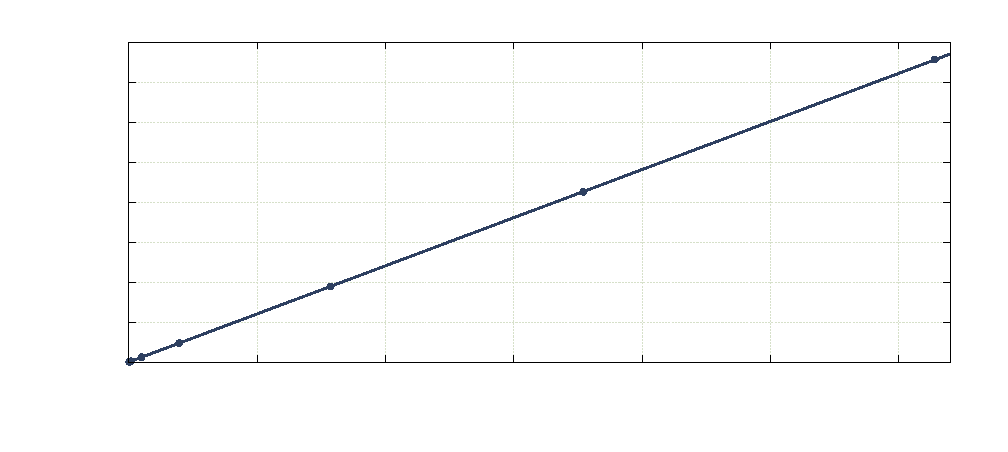
\includegraphics[trim=0 0 0.1cm 0, clip]{Graphs/2/Leak/Leak}}}%
    \gplfronttext
  \end{picture}%
\endgroup

		 	\caption[The estimated power loss vs leakage area.]{ The estimated power loss vs leakage area \cite{van2011sustaining}.}
		 	\label{fig: Leak losses}
		 \end{figure}
		 Air is often not easily detected through visual methods. In industry, a number of techniques are employed to detect air leaks. Pascoe \cite{Pascoe2016Masters} and van Tonder \cite{vanTonder2010Masters} summarised these strategies as follows:
		 \begin{itemize}
		 	\item Audible detection (Walk and report)
		 	\item Ultrasonic detection
		 	\item Detection through intelligent systems
		 	\item Pigging
		 	\item soap water and dyes
		 \end{itemize}
	 	 These methods can be time and resource intensive and many mines do not actively employ dedicated leakage detection repair teams. Marais \textit{et al} \cite{marais2009increased} investigated streamlining the leakage detection and repair process to increase energy savings through the use of \gls{calds}. The \gls{calds} system was developed to allow centralised mobile leakage reporting. Usage of the system resulted in increased leak detection rate with one mine reporting 24 leaks in a single month. It was noted in the study that there difficulty quantifying the actual energy savings of the leakage repairs due to other intervention occurring simultaneously.	
		 
		 \subsubsection{Underground control valves optimisation}
		 Many mines utilise automated valves at critical locations or levels in the compressed air network. These valves control the pressure, restricting airflow from that point in the air network. Restricting airflow reduces losses resultant from network inefficiencies and leaks.
		 \par 
		 Kleingeld and Marais \cite{kleingeld2010high} found that optimising control valve control on mining levels can conservatively lead to between 20\% on mines where no control valves are installed. For systems that already have some form of network control, between 10 and 15\% savings can conservatively be achieved.
		 \par 
		 From literature, the advantage of control valve optimisation is the significant savings that can be achieved with relatively short set-up up time. Savings can be achieved incrementally with each control valve installation. Studies did not look at accurate estimations of savings or the shaft pressure improvements that result from control valve optimisation.	 
		\subsubsection{Improving pneumatic rock drill efficiency}
		 Pneumatic rock drills are on of the largest air consumers in a mine. However Pneumatic drilling systems are convert energy very inefficiently. Replacing pneumatic drills with more efficient alternatives such as hydraulic or pneumatic drills would lead to large energy savings \cite{Pascoe2016Masters}**.  Alternatively improving the efficiency or pneumatic drilling can have a significant energy impact on the system, without the cost and safety concerns of alternative drilling technologies.
		 \par 
		  In a study by  Bester \textit{et al.} \cite{bester2013effect} looking at the effect of compressed air pressure on energy demand. Bester showed that between 2002 and 2013 compressed air and energy consumption per tonne of ore produced had steadily increased. This is illustrated  in \cref{fig: Compressed energy and air flow per ton}. 
		 The increase of air consumption per \gls{t} was a result of reduced air pressure at the mining areas. This causes the drilling rate to drop leading to higher air consumption. Pressure measurements as low as 300 \gls{kpa} were recorded in these areas. Before 2002 the drilling pressure at the mining section (stopes), was maintained above 500 \gls{kpa} at most mines. 
		 \par 
		 \begin{figure}[h]
		 	\centering
		 	% GNUPLOT: LaTeX picture with Postscript
\begingroup
  \makeatletter
  \providecommand\color[2][]{%
    \GenericError{(gnuplot) \space\space\space\@spaces}{%
      Package color not loaded in conjunction with
      terminal option `colourtext'%
    }{See the gnuplot documentation for explanation.%
    }{Either use 'blacktext' in gnuplot or load the package
      color.sty in LaTeX.}%
    \renewcommand\color[2][]{}%
  }%
  \providecommand\includegraphics[2][]{%
    \GenericError{(gnuplot) \space\space\space\@spaces}{%
      Package graphicx or graphics not loaded%
    }{See the gnuplot documentation for explanation.%
    }{The gnuplot epslatex terminal needs graphicx.sty or graphics.sty.}%
    \renewcommand\includegraphics[2][]{}%
  }%
  \providecommand\rotatebox[2]{#2}%
  \@ifundefined{ifGPcolor}{%
    \newif\ifGPcolor
    \GPcolortrue
  }{}%
  \@ifundefined{ifGPblacktext}{%
    \newif\ifGPblacktext
    \GPblacktextfalse
  }{}%
  % define a \g@addto@macro without @ in the name:
  \let\gplgaddtomacro\g@addto@macro
  % define empty templates for all commands taking text:
  \gdef\gplbacktext{}%
  \gdef\gplfronttext{}%
  \makeatother
  \ifGPblacktext
    % no textcolor at all
    \def\colorrgb#1{}%
    \def\colorgray#1{}%
  \else
    % gray or color?
    \ifGPcolor
      \def\colorrgb#1{\color[rgb]{#1}}%
      \def\colorgray#1{\color[gray]{#1}}%
      \expandafter\def\csname LTw\endcsname{\color{white}}%
      \expandafter\def\csname LTb\endcsname{\color{black}}%
      \expandafter\def\csname LTa\endcsname{\color{black}}%
      \expandafter\def\csname LT0\endcsname{\color[rgb]{1,0,0}}%
      \expandafter\def\csname LT1\endcsname{\color[rgb]{0,1,0}}%
      \expandafter\def\csname LT2\endcsname{\color[rgb]{0,0,1}}%
      \expandafter\def\csname LT3\endcsname{\color[rgb]{1,0,1}}%
      \expandafter\def\csname LT4\endcsname{\color[rgb]{0,1,1}}%
      \expandafter\def\csname LT5\endcsname{\color[rgb]{1,1,0}}%
      \expandafter\def\csname LT6\endcsname{\color[rgb]{0,0,0}}%
      \expandafter\def\csname LT7\endcsname{\color[rgb]{1,0.3,0}}%
      \expandafter\def\csname LT8\endcsname{\color[rgb]{0.5,0.5,0.5}}%
    \else
      % gray
      \def\colorrgb#1{\color{black}}%
      \def\colorgray#1{\color[gray]{#1}}%
      \expandafter\def\csname LTw\endcsname{\color{white}}%
      \expandafter\def\csname LTb\endcsname{\color{black}}%
      \expandafter\def\csname LTa\endcsname{\color{black}}%
      \expandafter\def\csname LT0\endcsname{\color{black}}%
      \expandafter\def\csname LT1\endcsname{\color{black}}%
      \expandafter\def\csname LT2\endcsname{\color{black}}%
      \expandafter\def\csname LT3\endcsname{\color{black}}%
      \expandafter\def\csname LT4\endcsname{\color{black}}%
      \expandafter\def\csname LT5\endcsname{\color{black}}%
      \expandafter\def\csname LT6\endcsname{\color{black}}%
      \expandafter\def\csname LT7\endcsname{\color{black}}%
      \expandafter\def\csname LT8\endcsname{\color{black}}%
    \fi
  \fi
    \setlength{\unitlength}{0.0500bp}%
    \ifx\gptboxheight\undefined%
      \newlength{\gptboxheight}%
      \newlength{\gptboxwidth}%
      \newsavebox{\gptboxtext}%
    \fi%
    \setlength{\fboxrule}{0.5pt}%
    \setlength{\fboxsep}{1pt}%
\begin{picture}(9360.00,4032.00)%
    \gplgaddtomacro\gplbacktext{%
      \colorrgb{0.42,0.42,0.42}%
      \put(682,924){\makebox(0,0)[r]{\strut{}$0$}}%
      \colorrgb{0.42,0.42,0.42}%
      \put(682,1230){\makebox(0,0)[r]{\strut{}$5$}}%
      \colorrgb{0.42,0.42,0.42}%
      \put(682,1536){\makebox(0,0)[r]{\strut{}$10$}}%
      \colorrgb{0.42,0.42,0.42}%
      \put(682,1842){\makebox(0,0)[r]{\strut{}$15$}}%
      \colorrgb{0.42,0.42,0.42}%
      \put(682,2148){\makebox(0,0)[r]{\strut{}$20$}}%
      \colorrgb{0.42,0.42,0.42}%
      \put(682,2453){\makebox(0,0)[r]{\strut{}$25$}}%
      \colorrgb{0.42,0.42,0.42}%
      \put(682,2759){\makebox(0,0)[r]{\strut{}$30$}}%
      \colorrgb{0.42,0.42,0.42}%
      \put(682,3065){\makebox(0,0)[r]{\strut{}$35$}}%
      \colorrgb{0.42,0.42,0.42}%
      \put(682,3371){\makebox(0,0)[r]{\strut{}$40$}}%
      \colorrgb{0.42,0.42,0.42}%
      \put(814,704){\makebox(0,0){\strut{}$2002$}}%
      \colorrgb{0.42,0.42,0.42}%
      \put(2025,704){\makebox(0,0){\strut{}$2004$}}%
      \colorrgb{0.42,0.42,0.42}%
      \put(3237,704){\makebox(0,0){\strut{}$2006$}}%
      \colorrgb{0.42,0.42,0.42}%
      \put(4448,704){\makebox(0,0){\strut{}$2008$}}%
      \colorrgb{0.42,0.42,0.42}%
      \put(5659,704){\makebox(0,0){\strut{}$2010$}}%
      \colorrgb{0.42,0.42,0.42}%
      \put(6871,704){\makebox(0,0){\strut{}$2012$}}%
      \colorrgb{0.42,0.42,0.42}%
      \put(8082,704){\makebox(0,0){\strut{}$2014$}}%
      \colorrgb{0.42,0.42,0.42}%
      \put(8214,924){\makebox(0,0)[l]{\strut{}$0$}}%
      \colorrgb{0.42,0.42,0.42}%
      \put(8214,1230){\makebox(0,0)[l]{\strut{}$50$}}%
      \colorrgb{0.42,0.42,0.42}%
      \put(8214,1536){\makebox(0,0)[l]{\strut{}$100$}}%
      \colorrgb{0.42,0.42,0.42}%
      \put(8214,1842){\makebox(0,0)[l]{\strut{}$150$}}%
      \colorrgb{0.42,0.42,0.42}%
      \put(8214,2148){\makebox(0,0)[l]{\strut{}$200$}}%
      \colorrgb{0.42,0.42,0.42}%
      \put(8214,2453){\makebox(0,0)[l]{\strut{}$250$}}%
      \colorrgb{0.42,0.42,0.42}%
      \put(8214,2759){\makebox(0,0)[l]{\strut{}$300$}}%
      \colorrgb{0.42,0.42,0.42}%
      \put(8214,3065){\makebox(0,0)[l]{\strut{}$350$}}%
      \colorrgb{0.42,0.42,0.42}%
      \put(8214,3371){\makebox(0,0)[l]{\strut{}$400$}}%
    }%
    \gplgaddtomacro\gplfronttext{%
      \csname LTb\endcsname%
      \put(176,2147){\rotatebox{-270}{\makebox(0,0){\strut{}kWh/t}}}%
      \put(8851,2147){\rotatebox{-270}{\makebox(0,0){\strut{}$m^3$/t}}}%
      \put(4448,374){\makebox(0,0){\strut{}Year}}%
      \put(4448,3701){\makebox(0,0){\strut{}Compressed air energy and Volume consumed per ton}}%
      \csname LTb\endcsname%
      \put(3593,173){\makebox(0,0)[r]{\strut{}Energy per Ton (kWh/t)}}%
      \csname LTb\endcsname%
      \put(7352,173){\makebox(0,0)[r]{\strut{}Volume per Ton ($m^3$/t)}}%
    }%
    \gplbacktext
    \put(0,0){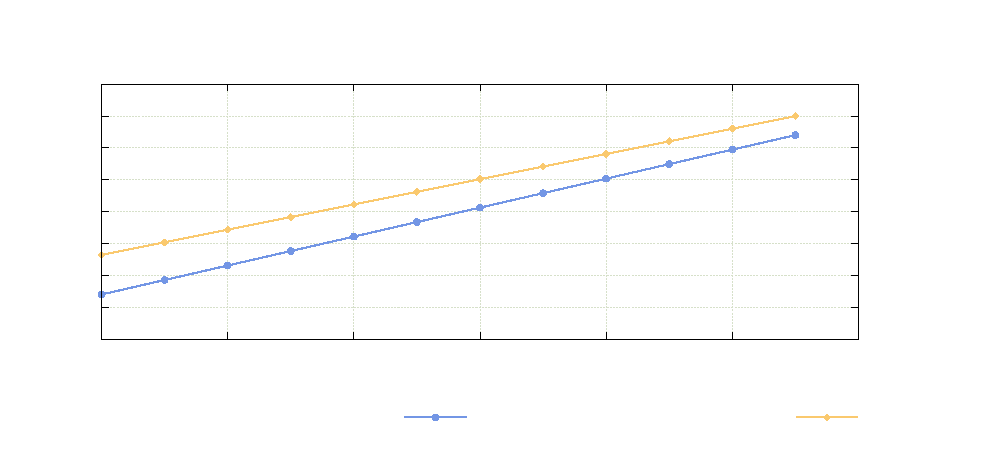
\includegraphics{Graphs/1/EVperT/EVperT}}%
    \gplfronttext
  \end{picture}%
\endgroup

		 	\caption[The Compressed air energy and flow consumed per T of ore produced.]{The Compressed air energy and flow consumed per T of ore produced. Adopted from Bester \textit{et al.} \cite{bester2013effect}.}
		 	\label{fig: Compressed energy and air flow per ton}
		 \end{figure}
		 From literature, it is shown that lowering the pressure reduces the efficiency and drill rate of rock drilling, leading to higher air consumption. Interventions that reduce systemic air losses or optimise supply can increase the pressure operating pressure. Increased pressure, during the drilling shift, may add more value than the energy cost savings that can be achieved at a lower pressure.
	\subsection{Summary}
\clearpage

\section{Use of simulations to identify improvements in mining systems}
	\subsection{Preamble}
	The value of simulation in  the mining industry has been shown through its use in \gls{dsm} initiatives. Simulation has been used to identify savings strategies for water reticulation cooling, compressed air and ventilation. This section will summarise the the work that has been done in industry. From this the successes and shortcomings of previous work will be discussed.
	
		\subsection{Estimating techniques used for energy savings on mining systems }
		Estimation of energy savings has been used in literature to obtain the potential energy impact that can be achieved for a system. Before new tools allowed for quick development of simplified simulation models, estimation techniques were frequently used to determine the feasibility of energy interventions on mining systems. The problem with an estimation approach is that they typically rely on simplified models with high resultant error.
		\par 
		- Snyman estimated improvements using historical data.\cite{Snyman2011Masters}\\
		- Marais estimation through simplified estimation, simulation \cite{Marais2012PhD},\cite{marais2013simplification}.
		
		\subsubsection{Benchmark modelling}
		Cilliers \cite{Cilliers2015PHD} developed \enquote{best practice models} using the \gls{cols} benchmarking method. These models provide an energy benchmark that can be used to identify the scope for energy improvements on a system. An example of a benchmark model for a mining compressed air system is shown in \cref{eq: COLS}. The model shows that energy required is dependent on the quantity of ore mined aswell as the the depth of the mine. \cite{Cilliers2015PHD} also developed benchmark models for mine cooling, water reticulation and ventilation systems.

		\begin{figure}[h!]
			\centering
			\fbox{% GNUPLOT: LaTeX picture with Postscript
\begingroup
  \makeatletter
  \providecommand\color[2][]{%
    \GenericError{(gnuplot) \space\space\space\@spaces}{%
      Package color not loaded in conjunction with
      terminal option `colourtext'%
    }{See the gnuplot documentation for explanation.%
    }{Either use 'blacktext' in gnuplot or load the package
      color.sty in LaTeX.}%
    \renewcommand\color[2][]{}%
  }%
  \providecommand\includegraphics[2][]{%
    \GenericError{(gnuplot) \space\space\space\@spaces}{%
      Package graphicx or graphics not loaded%
    }{See the gnuplot documentation for explanation.%
    }{The gnuplot epslatex terminal needs graphicx.sty or graphics.sty.}%
    \renewcommand\includegraphics[2][]{}%
  }%
  \providecommand\rotatebox[2]{#2}%
  \@ifundefined{ifGPcolor}{%
    \newif\ifGPcolor
    \GPcolortrue
  }{}%
  \@ifundefined{ifGPblacktext}{%
    \newif\ifGPblacktext
    \GPblacktextfalse
  }{}%
  % define a \g@addto@macro without @ in the name:
  \let\gplgaddtomacro\g@addto@macro
  % define empty templates for all commands taking text:
  \gdef\gplbacktext{}%
  \gdef\gplfronttext{}%
  \makeatother
  \ifGPblacktext
    % no textcolor at all
    \def\colorrgb#1{}%
    \def\colorgray#1{}%
  \else
    % gray or color?
    \ifGPcolor
      \def\colorrgb#1{\color[rgb]{#1}}%
      \def\colorgray#1{\color[gray]{#1}}%
      \expandafter\def\csname LTw\endcsname{\color{white}}%
      \expandafter\def\csname LTb\endcsname{\color{black}}%
      \expandafter\def\csname LTa\endcsname{\color{black}}%
      \expandafter\def\csname LT0\endcsname{\color[rgb]{1,0,0}}%
      \expandafter\def\csname LT1\endcsname{\color[rgb]{0,1,0}}%
      \expandafter\def\csname LT2\endcsname{\color[rgb]{0,0,1}}%
      \expandafter\def\csname LT3\endcsname{\color[rgb]{1,0,1}}%
      \expandafter\def\csname LT4\endcsname{\color[rgb]{0,1,1}}%
      \expandafter\def\csname LT5\endcsname{\color[rgb]{1,1,0}}%
      \expandafter\def\csname LT6\endcsname{\color[rgb]{0,0,0}}%
      \expandafter\def\csname LT7\endcsname{\color[rgb]{1,0.3,0}}%
      \expandafter\def\csname LT8\endcsname{\color[rgb]{0.5,0.5,0.5}}%
    \else
      % gray
      \def\colorrgb#1{\color{black}}%
      \def\colorgray#1{\color[gray]{#1}}%
      \expandafter\def\csname LTw\endcsname{\color{white}}%
      \expandafter\def\csname LTb\endcsname{\color{black}}%
      \expandafter\def\csname LTa\endcsname{\color{black}}%
      \expandafter\def\csname LT0\endcsname{\color{black}}%
      \expandafter\def\csname LT1\endcsname{\color{black}}%
      \expandafter\def\csname LT2\endcsname{\color{black}}%
      \expandafter\def\csname LT3\endcsname{\color{black}}%
      \expandafter\def\csname LT4\endcsname{\color{black}}%
      \expandafter\def\csname LT5\endcsname{\color{black}}%
      \expandafter\def\csname LT6\endcsname{\color{black}}%
      \expandafter\def\csname LT7\endcsname{\color{black}}%
      \expandafter\def\csname LT8\endcsname{\color{black}}%
    \fi
  \fi
    \setlength{\unitlength}{0.0500bp}%
    \ifx\gptboxheight\undefined%
      \newlength{\gptboxheight}%
      \newlength{\gptboxwidth}%
      \newsavebox{\gptboxtext}%
    \fi%
    \setlength{\fboxrule}{0.5pt}%
    \setlength{\fboxsep}{1pt}%
\begin{picture}(7000.00,5200.00)%
    \gplgaddtomacro\gplbacktext{%
      \colorrgb{0.00,0.00,0.00}%
      \put(936,1465){\makebox(0,0){\strut{}$0$}}%
      \colorrgb{0.00,0.00,0.00}%
      \put(1745,1325){\makebox(0,0){\strut{}$1$}}%
      \colorrgb{0.00,0.00,0.00}%
      \put(2555,1184){\makebox(0,0){\strut{}$2$}}%
      \colorrgb{0.00,0.00,0.00}%
      \put(3365,1043){\makebox(0,0){\strut{}$3$}}%
      \colorrgb{0.00,0.00,0.00}%
      \put(4174,903){\makebox(0,0){\strut{}$4$}}%
      \colorrgb{0.00,0.00,0.00}%
      \put(4600,965){\makebox(0,0){\strut{}$0$}}%
      \colorrgb{0.00,0.00,0.00}%
      \put(4850,1087){\makebox(0,0){\strut{}$20$}}%
      \colorrgb{0.00,0.00,0.00}%
      \put(5050,1208){\makebox(0,0){\strut{}$40$}}%
      \colorrgb{0.00,0.00,0.00}%
      \put(5300,1330){\makebox(0,0){\strut{}$60$}}%
      \colorrgb{0.00,0.00,0.00}%
      \put(5530,1452){\makebox(0,0){\strut{}$80$}}%
      \colorrgb{0.00,0.00,0.00}%
      \put(5770,1574){\makebox(0,0){\strut{}$100$}}%
      \colorrgb{0.00,0.00,0.00}%
      \put(6000,1695){\makebox(0,0){\strut{}$120$}}%
      \colorrgb{0.00,0.00,0.00}%
      \put(6230,1817){\makebox(0,0){\strut{}$140$}}%
      \colorrgb{0.00,0.00,0.00}%
      \put(6470,1939){\makebox(0,0){\strut{}$160$}}%
      \colorrgb{0.00,0.00,0.00}%
      \put(920,2210){\makebox(0,0)[r]{\strut{}$0$}}%
      \colorrgb{0.00,0.00,0.00}%
      \put(920,2470){\makebox(0,0)[r]{\strut{}$2$}}%
      \colorrgb{0.00,0.00,0.00}%
      \put(920,2729){\makebox(0,0)[r]{\strut{}$4$}}%
      \colorrgb{0.00,0.00,0.00}%
      \put(920,2988){\makebox(0,0)[r]{\strut{}$6$}}%
      \colorrgb{0.00,0.00,0.00}%
      \put(920,3248){\makebox(0,0)[r]{\strut{}$8$}}%
      \colorrgb{0.00,0.00,0.00}%
      \put(920,3508){\makebox(0,0)[r]{\strut{}$10$}}%
    }%
    \gplgaddtomacro\gplfronttext{%
    	\csname LTb\endcsname%
    	\put(5456,200){\makebox(0,0)[r]{\strut{}$E_{comp} = 1.51\cdot Z + 33.36\cdot T - 1930.21$}}%  	
    	\csname LTb\endcsname%
    	\put(6000,1400){\rotatebox{28}{\makebox(0,0){\strut{} T - Mined ore ($kT$)}}}%
    	\put(2100,1000){\rotatebox{-9}{\makebox(0,0){\strut{}Z - Mine depth ($km$)}}}%
    	\put(600,2858){\rotatebox{-270}{\makebox(0,0){\strut{}Benchmark energy (GWhr)}}}%
    }%
    \gplbacktext
    \put(0,0){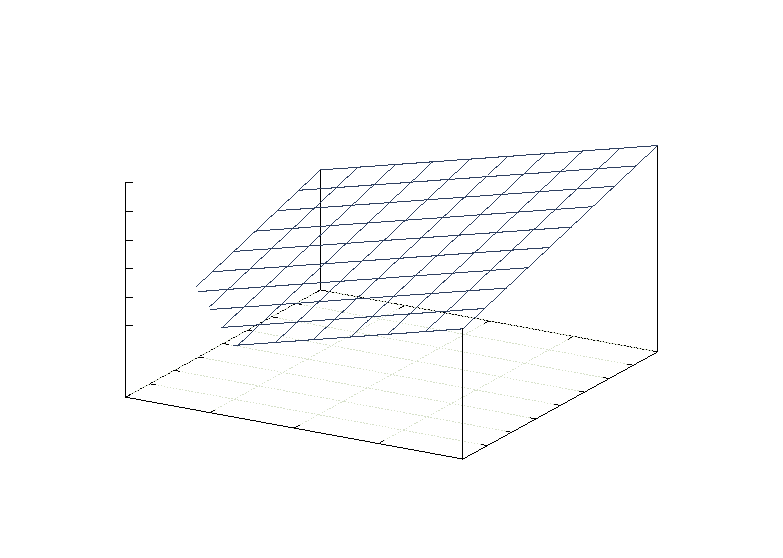
\includegraphics[trim=0 -0.51cm 0 0 ]{Graphs/2/Benchmark/Benchmark}}%
    \gplfronttext
  \end{picture}%
\endgroup
}
			\caption{ }
			\label{fig: 3D Benchmark}
		\end{figure}
	%%%%%%%%%%%%%%%%%%%%%%%%%% Equation %%%%%%%%%%%%%%%%%%%%%%%%%%%%%
	%	\begin{equation}
	%	\label{eq: COLS}
	%	E_{comp} = 1.51\cdot Z + 33.36\cdot T - 1930.21
	%	\end{equation}
	%	Where: 
	%		\begin{table}[h!]
	%			\centering
	%			\begin{tabular}{ll}
	%				$E_{comp}$ & Benchmark energy (MWhr)  \\
	%				$T$ & Mined ore ($kT$) \\
	%				$Z$ & Mine depth ($m$) \\
	%			\end{tabular} 
	%		\end{table}
	%%%%%%%%%%%%%%%%%%%%%%%%%%%%%%%%%%%%%%%%%%%%%%%%%%%%%%%%%%%%%%%%%%
	\subsection{Value of simulation in mining DSM}
	Van Niekerk \cite{van2013value},\cite{vanNiekerk2012Value} investigated the value of simulation models in mine \gls{dsm} projects. Van Niekerk developed simulation models for compressed air and water reticulation systems using KYPipes's gas simulation engine. \\
	
	\subsubsection{Mine cooling systems}
	Simulation has been used in studies as a tool to improve mine cooling. Holman \cite{Holman2014Masters} investigated improvements to mine cooling systems that improve performance and efficiency. In the study \cite{Holman2014Masters}  used simplified \gls{ptb}  simulation models to investigate cooling interventions.
	\par 
	The scenario Holman simulated showed potential  average power reduction of 136 kW  which would lead to an annual energy cost saving of R0.55M. The study could be improved by increasing accuracy of the simulation. Power difference of as high as 31\% between the simulation and actual were observed for some time periods.
	\subsubsection{Mine de-watering systems}
	
	\subsubsection{Mine compressed air systems}
		
	\subsection{Simulation procedures}
		- Philip
		- Kriel masters\\
		\subsubsection{Periodic simulation}
 	\subsection{Simulation model verification strategies}
 	From literature, methods of verifying simulation were analysed. Most studies utilised a comparison calculation strategy to calculate a model accuracy or error. Two calculation methods identified were \emph{Average difference method} and \emph{average percentage difference}. 
 		\subsubsection{Average difference method}
 			The average difference method looks at the sum for a simulated output for all time-steps in the period. This same is done for the actual system value. The error \% is then calculated as shown in \cref{eq: Average difference}
 			
 			\begin{equation}
 				\label{eq: Average difference}
 				Err_{\%} = \left| \dfrac{ \sum_{n}^{N}{ \left( \dfrac{A_{n}}{N} \right)}  - \sum_{n}^{N}{ \left( \dfrac{M_{n}}{N} \right) } }{ \sum_{n}^{N}{ \left( \dfrac{A_{n}}{N} \right) } } \right|
 			\end{equation}
 			Where: 
 				\begin{table}[h!]
 					\centering
 					\begin{tabular}{cl}
 						$A$ & Actual system parameter \\
 						$M$ & Model parameter \\
 						$n$ & sample \\
 						$N$ & Number of samples in simulation period \\
 					\end{tabular} 
 				\end{table}	
 		\subsubsection{Relative error method}
 		The relative error method follows a similar calculation as in the Average difference method. However, as shown in \cref{eq: Relative error}, the error is calculated for each sample in the period is calculated, the average of the error is then calculated.
 			
 			\begin{equation}
 			\label{eq: Relative error}
 			Err_{\%} = \dfrac{\sum_{n}^{N}{\left|\dfrac{A_{n} - M_{n}}{A_{n}}\right| }}{N}
 			\end{equation}
 			Where: 
 			\begin{table}[h!]
 				\centering
 				\begin{tabular}{cl}
 					$A$ & Actual system parameter \\
 					$M$ & Model parameter \\
 					$n$ & sample \\
 					$N$ & Number of samples in simulation period \\
 				\end{tabular} 
 			\end{table}	
 		Yu-jie Xu \cite{xu2016modeling}
 		\par 
 		The difference between the two verification strategies is best illustrate using an example. Figure \cref{fig:Philipp Diffeence verify} Shows a comparison between a simulation model's output power and and the actual power of the system over a 24 hour period. In the study \cite{Mare2016PhD} used the average \% difference method utilising the average power over the entire period for the two parameters. This lead to a calculated Average Err of 1.17\%. However if the Relative error method, \cref{eq: Relative error}, is applied to the same data, the resultant error is then 15.2 \%. 
 		
 		philip phd \cite{Mare2016PhD}
 		
 	\begin{figure}[h!]
 		\centering
 		% GNUPLOT: LaTeX picture with Postscript
\begingroup
  \makeatletter
  \providecommand\color[2][]{%
    \GenericError{(gnuplot) \space\space\space\@spaces}{%
      Package color not loaded in conjunction with
      terminal option `colourtext'%
    }{See the gnuplot documentation for explanation.%
    }{Either use 'blacktext' in gnuplot or load the package
      color.sty in LaTeX.}%
    \renewcommand\color[2][]{}%
  }%
  \providecommand\includegraphics[2][]{%
    \GenericError{(gnuplot) \space\space\space\@spaces}{%
      Package graphicx or graphics not loaded%
    }{See the gnuplot documentation for explanation.%
    }{The gnuplot epslatex terminal needs graphicx.sty or graphics.sty.}%
    \renewcommand\includegraphics[2][]{}%
  }%
  \providecommand\rotatebox[2]{#2}%
  \@ifundefined{ifGPcolor}{%
    \newif\ifGPcolor
    \GPcolortrue
  }{}%
  \@ifundefined{ifGPblacktext}{%
    \newif\ifGPblacktext
    \GPblacktextfalse
  }{}%
  % define a \g@addto@macro without @ in the name:
  \let\gplgaddtomacro\g@addto@macro
  % define empty templates for all commands taking text:
  \gdef\gplbacktext{}%
  \gdef\gplfronttext{}%
  \makeatother
  \ifGPblacktext
    % no textcolor at all
    \def\colorrgb#1{}%
    \def\colorgray#1{}%
  \else
    % gray or color?
    \ifGPcolor
      \def\colorrgb#1{\color[rgb]{#1}}%
      \def\colorgray#1{\color[gray]{#1}}%
      \expandafter\def\csname LTw\endcsname{\color{white}}%
      \expandafter\def\csname LTb\endcsname{\color{black}}%
      \expandafter\def\csname LTa\endcsname{\color{black}}%
      \expandafter\def\csname LT0\endcsname{\color[rgb]{1,0,0}}%
      \expandafter\def\csname LT1\endcsname{\color[rgb]{0,1,0}}%
      \expandafter\def\csname LT2\endcsname{\color[rgb]{0,0,1}}%
      \expandafter\def\csname LT3\endcsname{\color[rgb]{1,0,1}}%
      \expandafter\def\csname LT4\endcsname{\color[rgb]{0,1,1}}%
      \expandafter\def\csname LT5\endcsname{\color[rgb]{1,1,0}}%
      \expandafter\def\csname LT6\endcsname{\color[rgb]{0,0,0}}%
      \expandafter\def\csname LT7\endcsname{\color[rgb]{1,0.3,0}}%
      \expandafter\def\csname LT8\endcsname{\color[rgb]{0.5,0.5,0.5}}%
    \else
      % gray
      \def\colorrgb#1{\color{black}}%
      \def\colorgray#1{\color[gray]{#1}}%
      \expandafter\def\csname LTw\endcsname{\color{white}}%
      \expandafter\def\csname LTb\endcsname{\color{black}}%
      \expandafter\def\csname LTa\endcsname{\color{black}}%
      \expandafter\def\csname LT0\endcsname{\color{black}}%
      \expandafter\def\csname LT1\endcsname{\color{black}}%
      \expandafter\def\csname LT2\endcsname{\color{black}}%
      \expandafter\def\csname LT3\endcsname{\color{black}}%
      \expandafter\def\csname LT4\endcsname{\color{black}}%
      \expandafter\def\csname LT5\endcsname{\color{black}}%
      \expandafter\def\csname LT6\endcsname{\color{black}}%
      \expandafter\def\csname LT7\endcsname{\color{black}}%
      \expandafter\def\csname LT8\endcsname{\color{black}}%
    \fi
  \fi
    \setlength{\unitlength}{0.0500bp}%
    \ifx\gptboxheight\undefined%
      \newlength{\gptboxheight}%
      \newlength{\gptboxwidth}%
      \newsavebox{\gptboxtext}%
    \fi%
    \setlength{\fboxrule}{0.5pt}%
    \setlength{\fboxsep}{1pt}%
\begin{picture}(9360.00,4536.00)%
    \gplgaddtomacro\gplbacktext{%
      \colorrgb{0.00,0.00,0.00}%
      \put(682,1584){\makebox(0,0)[r]{\strut{}$0$}}%
      \colorrgb{0.00,0.00,0.00}%
      \put(682,1853){\makebox(0,0)[r]{\strut{}$1$}}%
      \colorrgb{0.00,0.00,0.00}%
      \put(682,2121){\makebox(0,0)[r]{\strut{}$2$}}%
      \colorrgb{0.00,0.00,0.00}%
      \put(682,2390){\makebox(0,0)[r]{\strut{}$3$}}%
      \colorrgb{0.00,0.00,0.00}%
      \put(682,2659){\makebox(0,0)[r]{\strut{}$4$}}%
      \colorrgb{0.00,0.00,0.00}%
      \put(682,2927){\makebox(0,0)[r]{\strut{}$5$}}%
      \colorrgb{0.00,0.00,0.00}%
      \put(682,3196){\makebox(0,0)[r]{\strut{}$6$}}%
      \colorrgb{0.00,0.00,0.00}%
      \put(682,3465){\makebox(0,0)[r]{\strut{}$7$}}%
      \colorrgb{0.00,0.00,0.00}%
      \put(682,3734){\makebox(0,0)[r]{\strut{}$8$}}%
      \colorrgb{0.00,0.00,0.00}%
      \put(682,4002){\makebox(0,0)[r]{\strut{}$9$}}%
      \colorrgb{0.00,0.00,0.00}%
      \put(682,4271){\makebox(0,0)[r]{\strut{}$10$}}%
      \colorrgb{0.00,0.00,0.00}%
      \put(1286,1364){\makebox(0,0){\strut{}02:00}}%
      \colorrgb{0.00,0.00,0.00}%
      \put(1916,1364){\makebox(0,0){\strut{}04:00}}%
      \colorrgb{0.00,0.00,0.00}%
      \put(2546,1364){\makebox(0,0){\strut{}06:00}}%
      \colorrgb{0.00,0.00,0.00}%
      \put(3176,1364){\makebox(0,0){\strut{}08:00}}%
      \colorrgb{0.00,0.00,0.00}%
      \put(3805,1364){\makebox(0,0){\strut{}10:00}}%
      \colorrgb{0.00,0.00,0.00}%
      \put(4435,1364){\makebox(0,0){\strut{}12:00}}%
      \colorrgb{0.00,0.00,0.00}%
      \put(5065,1364){\makebox(0,0){\strut{}14:00}}%
      \colorrgb{0.00,0.00,0.00}%
      \put(5695,1364){\makebox(0,0){\strut{}16:00}}%
      \colorrgb{0.00,0.00,0.00}%
      \put(6325,1364){\makebox(0,0){\strut{}18:00}}%
      \colorrgb{0.00,0.00,0.00}%
      \put(6954,1364){\makebox(0,0){\strut{}20:00}}%
      \colorrgb{0.00,0.00,0.00}%
      \put(7584,1364){\makebox(0,0){\strut{}22:00}}%
      \colorrgb{0.00,0.00,0.00}%
      \put(8214,1364){\makebox(0,0){\strut{}00:00}}%
      \colorrgb{0.00,0.00,0.00}%
      \put(8346,1584){\makebox(0,0)[l]{\strut{}$0$}}%
      \colorrgb{0.00,0.00,0.00}%
      \put(8346,1853){\makebox(0,0)[l]{\strut{}$1$}}%
      \colorrgb{0.00,0.00,0.00}%
      \put(8346,2121){\makebox(0,0)[l]{\strut{}$2$}}%
      \colorrgb{0.00,0.00,0.00}%
      \put(8346,2390){\makebox(0,0)[l]{\strut{}$3$}}%
      \colorrgb{0.00,0.00,0.00}%
      \put(8346,2659){\makebox(0,0)[l]{\strut{}$4$}}%
      \colorrgb{0.00,0.00,0.00}%
      \put(8346,2927){\makebox(0,0)[l]{\strut{}$5$}}%
      \colorrgb{0.00,0.00,0.00}%
      \put(8346,3196){\makebox(0,0)[l]{\strut{}$6$}}%
      \colorrgb{0.00,0.00,0.00}%
      \put(8346,3465){\makebox(0,0)[l]{\strut{}$7$}}%
      \colorrgb{0.00,0.00,0.00}%
      \put(8346,3734){\makebox(0,0)[l]{\strut{}$8$}}%
      \colorrgb{0.00,0.00,0.00}%
      \put(8346,4002){\makebox(0,0)[l]{\strut{}$9$}}%
      \colorrgb{0.00,0.00,0.00}%
      \put(8346,4271){\makebox(0,0)[l]{\strut{}$10$}}%
      \csname LTb\endcsname%
      \put(1024,3000){\makebox(0,0)[l]{\strut{}\shortstack{Residual \\ difference}}}%
      \put(1024,1745){\makebox(0,0)[l]{\strut{}MAE}}%
      \put(1024,2014){\makebox(0,0)[l]{\strut{}MSE}}%
    }%
    \gplgaddtomacro\gplfronttext{%
      \csname LTb\endcsname%
      \put(176,2927){\rotatebox{-270}{\makebox(0,0){\strut{}Power $(MW)$}}}%
      \put(8851,2600){\rotatebox{-270}{\makebox(0,0){\strut{} Relative $Err_{\%} $}}}%
      \put(4514,1034){\makebox(0,0){\strut{}Time of use}}%
      \csname LTb\endcsname%
      \put(3659,833){\makebox(0,0)[r]{\strut{}AE \%}}%
      \csname LTb\endcsname%
      \put(3659,613){\makebox(0,0)[r]{\strut{}SE \%}}%
      \csname LTb\endcsname%
      \put(3659,393){\makebox(0,0)[r]{\strut{}MAE \%}}%
      \csname LTb\endcsname%
      \put(3659,173){\makebox(0,0)[r]{\strut{}MSE \%}}%
      \csname LTb\endcsname%
      \put(6890,833){\makebox(0,0)[r]{\strut{}Actual power}}%
      \csname LTb\endcsname%
      \put(6890,613){\makebox(0,0)[r]{\strut{}Simulated power}}%
      \csname LTb\endcsname%
      \put(6890,393){\makebox(0,0)[r]{\strut{}Average Actual}}%
      \csname LTb\endcsname%
      \put(6890,173){\makebox(0,0)[r]{\strut{}Average Simulation}}%
    }%
    \gplbacktext
    \put(0,0){\fbox{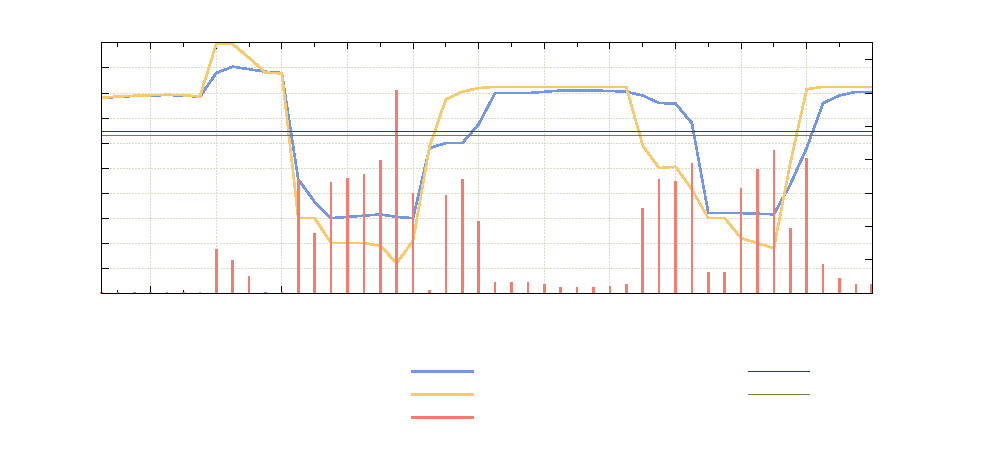
\includegraphics[trim=0 0 0.1cm 0, clip]{Graphs/2/Verification/Verification}}}%
    
    \gplfronttext
  \end{picture}%
\endgroup

 		\caption[Example of simulation error calculation.]{Example of simulation error calculation. Adapted from Marè \cite{Mare2016PhD}}
 		\label{fig:Philipp Diffeence verify}
 	\end{figure}
 

 	\subsubsection{Verification in previous studies}
 	Previous studies used verified there simulations through different methods and varying degrees of precision. \\
 	\begin{table}[h]
 		\centering
 		\begin{tabular}{p{5cm}ccr}
 			\hline
 			Study & Year & Verification method & Accepted margin\\
 			\hhline{====}
 			Holman \cite{Holman2014Masters} & 2014 & Average \% difference & Not specified  \\
 			van Niekerk \cite{vanNiekerk2012Value} & 1900 & Average \% difference & 5\% difference \\
 			Kriel \cite{Marais2012PhD} &  1900 & Average \% difference & 5\% difference \\
 			Pascoe \cite{Pascoe2016Masters} & 1900 & Average \% difference & 5\% difference \\	
 			Mare \cite{Mare2016PhD} & 1900 & Average \% difference & 5\% difference  \\
 			Marius \cite{Marais2012PhD} & 1900 & Average \% difference & 5\% difference\\	
 			Snyman	\cite{Snyman2011Masters} & 1900 & Average \% difference & 5\% difference\\	
 			Yu-jie-Xu \cite{xu2016modeling}& 1900 & relative \% error & 5\%  error\\	
 			Peach \cite{Peach2016Masters}& 2016 & Average \% difference & 5\% relative error\\
 			\hline
 		\end{tabular} 
 		\caption{Simulation verification methods that were implemented in previous studies.}
 		\label{table: Verification studies}
 	\end{table}
\clearpage	
\section{Use of simulation in compressed air system optimisation}
	

	\subsubsection{Simulations on compressed air systems}
		- Pascoe 
		- van Tonder
		- kriel
		- Mare
		- De Coning -  simulations to investigate the opportunity to optimise the control strategy of a compressed air network by rescheduling the compressors.
	\subsection{Summary}
	\label{Shortcomings of previous work}
		\clearpage	
\section{Conclusion}